\documentclass{article}
\usepackage{tikz}
\usetikzlibrary{shapes.geometric, arrows.meta, positioning}
\title{Blockchain-based Certificate Verification Application}
\author{}
\date{July 2025}

\begin{document}

\maketitle

\section{Introduction}
This document describes a web application that leverages blockchain technology and smart contracts to provide secure, transparent, and tamper-proof certificate verification. The application allows users to verify academic certificates by querying a blockchain-based smart contract and to download the corresponding certificate file from IPFS (InterPlanetary File System).

\section{System Overview}
The application consists of the following main components:
\begin{itemize}
    \item \textbf{Frontend:} A web interface where users can enter a certificate hash, complete a CAPTCHA, and verify the certificate. Upon successful verification, users can enter the IPFS CID to download the certificate PDF.
    \item \textbf{Backend:} A server that interacts with the blockchain smart contract and IPFS, exposing RESTful endpoints for verification and file download.
    \item \textbf{Blockchain Smart Contract:} A deployed contract that stores certificate data (issuer, student, timestamp, revocation status, and IPFS hash) and provides verification logic.
    \item \textbf{IPFS:} A decentralized file storage system where the actual certificate PDFs are stored and retrieved using their CIDs.
\end{itemize}

\section{Application Flow}
The typical flow for a user verifying and downloading a certificate is as follows:
\begin{enumerate}
    \item User enters the certificate hash and completes the CAPTCHA on the frontend.
    \item The frontend sends a verification request to the backend.
    \item The backend queries the smart contract on the blockchain to verify the certificate and retrieve its metadata.
    \item The backend returns the verification result to the frontend.
    \item If the certificate is valid, the user is prompted to enter the IPFS CID.
    \item The user enters the IPFS CID and clicks the download button.
    \item The frontend requests the backend to fetch the PDF from IPFS and provide it for download.
\end{enumerate}

\section{Flowchart}

\begin{center}
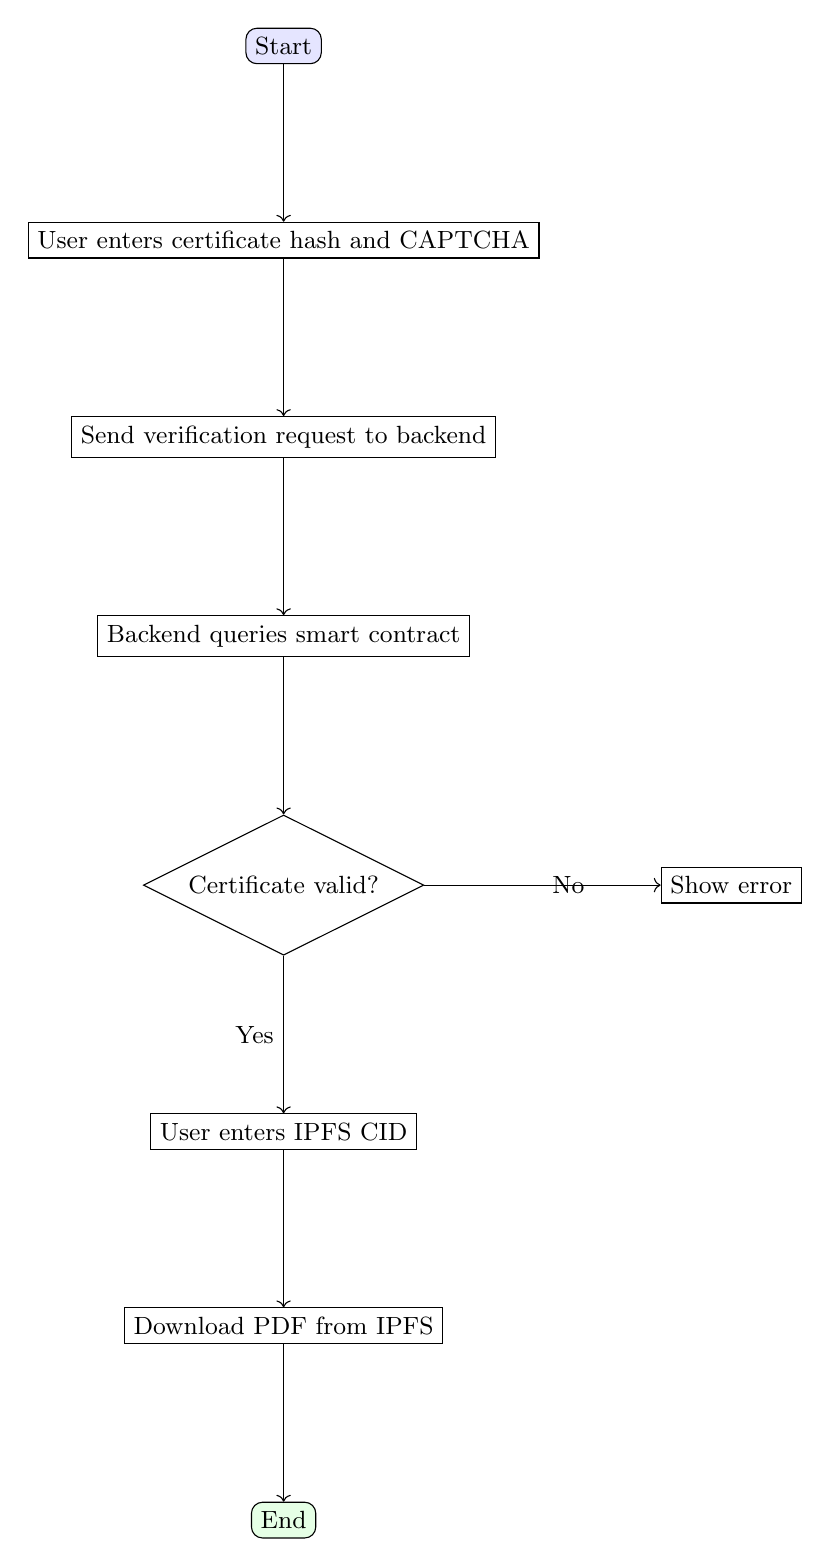
\begin{tikzpicture}[node distance=2cm, every node/.style={font=\small}]
  % Nodes
  \node (start) [rectangle, draw, rounded corners, fill=blue!10] {Start};
  \node (input) [rectangle, draw, below=of start] {User enters certificate hash and CAPTCHA};
  \node (verify) [rectangle, draw, below=of input] {Send verification request to backend};
  \node (contract) [rectangle, draw, below=of verify] {Backend queries smart contract};
  \node (result) [diamond, draw, aspect=2, below=of contract] {Certificate valid?};
  \node (fail) [rectangle, draw, right=3cm of result] {Show error};
  \node (cid) [rectangle, draw, below=of result] {User enters IPFS CID};
  \node (download) [rectangle, draw, below=of cid] {Download PDF from IPFS};
  \node (end) [rectangle, draw, rounded corners, below=of download, fill=green!10] {End};

  % Arrows
  \draw[->] (start) -- (input);
  \draw[->] (input) -- (verify);
  \draw[->] (verify) -- (contract);
  \draw[->] (contract) -- (result);
  \draw[->] (result) -- node[right] {No} (fail);
  \draw[->] (result) -- node[left] {Yes} (cid);
  \draw[->] (cid) -- (download);
  \draw[->] (download) -- (end);
\end{tikzpicture}
\end{center}

\section{Project Description}
This project implements a blockchain-based certificate management and verification system. It leverages smart contracts to securely issue, store, and verify academic certificates. The system involves three main actors:
\begin{itemize}
    \item \textbf{Issuer:} An authorized institution or entity that creates and issues certificates to students. The issuer interacts with the smart contract to register new certificates on the blockchain, associating them with student identities and storing the certificate file on IPFS.
    \item \textbf{Student:} The recipient of the certificate. Students can retrieve their certificate's IPFS CID and share it with third parties for verification. They can also check the status of their certificate (e.g., if it has been revoked).
    \item \textbf{Verifier:} Any third party (such as an employer or another institution) who wishes to verify the authenticity of a certificate. The verifier uses the web portal to check the certificate's validity and download the associated PDF from IPFS.
\end{itemize}

\section{User Flows}
\subsection{Issuer Flow}
\begin{enumerate}
    \item Issuer logs into the backend/admin portal.
    \item Fills in student and certificate details.
    \item Uploads the certificate PDF, which is stored on IPFS and returns a CID.
    \item The smart contract is called to register the certificate, storing metadata (issuer, student, timestamp, IPFS CID, etc.) on the blockchain.
    \item Issuer receives confirmation and can share the certificate hash and IPFS CID with the student.
\end{enumerate}

\subsection{Student Flow}
\begin{enumerate}
    \item Student receives the certificate hash and IPFS CID from the issuer.
    \item Student can use the web portal to verify the certificate's authenticity and status by entering the hash.
    \item Student can download the certificate PDF from IPFS using the CID.
    \item Student can share the hash and CID with verifiers.
\end{enumerate}

\subsection{Verifier Flow}
\begin{enumerate}
    \item Verifier accesses the public verification portal.
    \item Enters the certificate hash and completes CAPTCHA.
    \item The portal queries the smart contract for certificate metadata and status.
    \item If valid, the verifier enters the IPFS CID to download the PDF.
    \item The verifier reviews the certificate and its metadata.
\end{enumerate}

\section{Comprehensive Application Flowchart}

\begin{center}
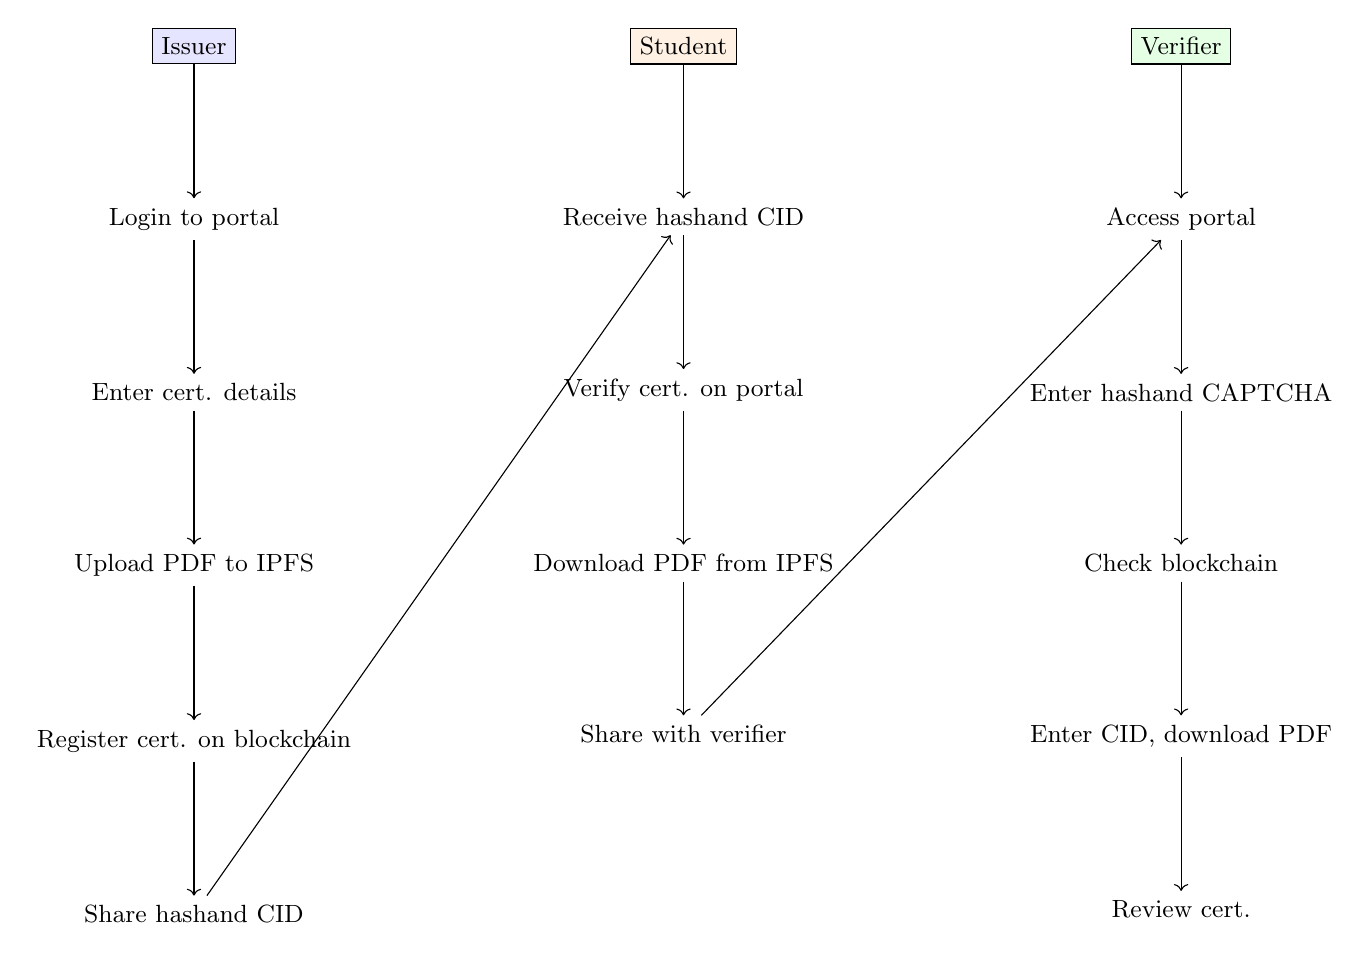
\begin{tikzpicture}[node distance=1.7cm, every node/.style={font=\small}]
  % Actors
  \node (issuer) [rectangle, draw, fill=blue!10] {Issuer};
  \node (student) [rectangle, draw, right=5cm of issuer, fill=orange!10] {Student};
  \node (verifier) [rectangle, draw, right=5cm of student, fill=green!10] {Verifier};

  % Issuer flow
  \node (issue1) [below=of issuer] {Login to portal};
  \node (issue2) [below=of issue1] {Enter cert. details};
  \node (issue3) [below=of issue2] {Upload PDF to IPFS};
  \node (issue4) [below=of issue3] {Register cert. on blockchain};
  \node (issue5) [below=of issue4] {Share hash \\ and CID};

  % Student flow
  \node (stud1) [below=of student] {Receive hash \\ and CID};
  \node (stud2) [below=of stud1] {Verify cert. on portal};
  \node (stud3) [below=of stud2] {Download PDF from IPFS};
  \node (stud4) [below=of stud3] {Share with verifier};

  % Verifier flow
  \node (ver1) [below=of verifier] {Access portal};
  \node (ver2) [below=of ver1] {Enter hash \\ and CAPTCHA};
  \node (ver3) [below=of ver2] {Check blockchain};
  \node (ver4) [below=of ver3] {Enter CID, download PDF};
  \node (ver5) [below=of ver4] {Review cert.};

  % Connect Issuer to Student
  \draw[->] (issue5) -- (stud1);
  % Connect Student to Verifier
  \draw[->] (stud4) -- (ver1);

  % Issuer vertical
  \draw[->] (issuer) -- (issue1);
  \draw[->] (issue1) -- (issue2);
  \draw[->] (issue2) -- (issue3);
  \draw[->] (issue3) -- (issue4);
  \draw[->] (issue4) -- (issue5);

  % Student vertical
  \draw[->] (student) -- (stud1);
  \draw[->] (stud1) -- (stud2);
  \draw[->] (stud2) -- (stud3);
  \draw[->] (stud3) -- (stud4);

  % Verifier vertical
  \draw[->] (verifier) -- (ver1);
  \draw[->] (ver1) -- (ver2);
  \draw[->] (ver2) -- (ver3);
  \draw[->] (ver3) -- (ver4);
  \draw[->] (ver4) -- (ver5);
\end{tikzpicture}
\end{center}

\section{Tools, Frameworks, and Libraries}

\subsection{List of Technologies}
\begin{itemize}
    \item \textbf{Python} -- Main backend programming language.
    \item \textbf{Django} -- Web framework for backend REST API and admin portal.
    \item \textbf{Django REST Framework} -- Toolkit for building Web APIs in Django.
    \item \textbf{Web3.py} -- Python library for interacting with Ethereum blockchain and smart contracts.
    \item \textbf{Solidity} -- Language for writing smart contracts deployed on Ethereum-compatible blockchains.
    \item \textbf{Ganache} -- Local Ethereum blockchain for development and testing.
    \item \textbf{IPFS (InterPlanetary File System)} -- Decentralized file storage for certificate PDFs.
    \item \textbf{React} -- JavaScript library for building the frontend user interface.
    \item \textbf{Elastic UI (EUI)} -- React component library for frontend UI elements.
    \item \textbf{Axios} -- Promise-based HTTP client for making API requests from the frontend.
    \item \textbf{reCAPTCHA} -- Google service for bot/spam protection on the frontend.
    \item \textbf{Docker} -- Containerization platform for deploying backend, frontend, and IPFS nodes.
    \item \textbf{SQLite} -- Lightweight database for development and testing.
    \item \textbf{Redis} -- In-memory data store, used for caching or task queues.
    \item \textbf{Celery} -- Distributed task queue for background jobs in Python.
    \item \textbf{Node.js} -- JavaScript runtime for frontend tooling and scripts.
    \item \textbf{TypeScript} -- Typed superset of JavaScript for frontend codebase.
    \item \textbf{Babel} -- JavaScript compiler for transpiling modern JS/TS code.
    \item \textbf{Jest} -- JavaScript testing framework for frontend tests.
    \item \textbf{Pytest} -- Python testing framework for backend tests.
\end{itemize}

\subsection{Explanation of Technologies}
\begin{description}
    \item[Python \,\&\, Django] Used for the backend REST API, business logic, and admin portal. Django REST Framework simplifies API creation and management.
    \item[Web3.py] Enables the backend to interact with Ethereum smart contracts for certificate registration and verification.
    \item[Solidity] The language used to write the smart contract that manages certificate data on the blockchain.
    \item[Ganache] Provides a local blockchain for safe development and testing of smart contracts.
    \item[IPFS] Stores certificate PDFs in a decentralized way, referenced by their CID in the smart contract.
    \item[React \,\&\, Elastic UI] Used to build a responsive, user-friendly frontend for students, issuers, and verifiers.
    \item[Axios] Handles HTTP requests from the frontend to the backend API.
    \item[reCAPTCHA] Protects the public verification portal from bots and spam.
    \item[Docker] Ensures consistent deployment and easy orchestration of backend, frontend, and IPFS services.
    \item[SQLite] Used as a simple database for development; can be replaced with PostgreSQL or MySQL in production.
    \item[Redis \,\&\, Celery] Used for caching and background task processing (e.g., sending notifications, handling uploads).
    \item[Node.js, TypeScript, Babel] Provide a modern, type-safe, and maintainable frontend development environment.
    \item[Jest \,\&\, Pytest] Used for automated testing of frontend and backend code, respectively.
\end{description}

\section{Conclusion}
This application demonstrates a practical use of blockchain and smart contracts for secure certificate verification, ensuring data integrity and transparency. The integration with IPFS further decentralizes storage, making the system robust and tamper-resistant.

\end{document}
